\documentclass[a4paper,12pt]{article}

% Configuração de idioma e codificação
\usepackage[utf8]{inputenc}
\usepackage[T1]{fontenc}
\usepackage[brazil]{babel}

% Layout da página
\usepackage[a4paper, margin=0.8in]{geometry}
\usepackage{setspace}
\setstretch{1.5} % Espaçamento entre linhas

\usepackage{amsmath, bm} % Pacotes matemáticos
\usepackage{graphicx} % Inclusão de imagens
\usepackage{caption} % Estilização de legendas
\usepackage{fancyhdr} % Personalização de cabeçalhos e rodapés
\usepackage{titlesec} % Personalização de títulos de seção
\usepackage{xcolor} % Cores para textos e seções
\usepackage{hyperref} % Links clicáveis
\usepackage{background} % Fundo para a página de título
\usepackage{placeins} % Controle de posicionamento de floats (FloatBarrier)
\usepackage{pdfpages}
\usepackage{enumitem}
% Ensure the package is loaded correctly for \floatbarrier

\hypersetup{
    colorlinks=true,
    linkcolor=red,
    urlcolor=red,
    citecolor=red
}

% Personalização dos títulos
\titleformat{\section}{\Large\bfseries\color{black}}{\thesection}{1em}{}
\titleformat{\subsection}{\large\bfseries\color{black}}{\thesubsection}{1em}{}

% Cabeçalhos e Rodapés
\pagestyle{fancy}
\fancyhf{}
\fancyhead[R]{
\includegraphics[width=2cm]{ITA.png}} % Logo no topo direito
\fancyhead[L]{\textbf{Instituto Tecnológico de Aeronáutica (ITA)}}
\fancyfoot[L]{Leonardo Peres Dias}
\fancyfoot[R]{\thepage}

% Informações do título
\title{
    \textbf{Inteligência Artificial para Robótica Móvel CT-213}\\
    \Large Instituto Tecnológico de Aeronáutica 

    \textbf{Relatório do Laboratório 11 -  Aprendizado por Reforço Livre de Modelo}\\
}
\author{
    Leonardo Peres Dias 
}
\date{\today}

% Configuração do fundo (marca d'água apenas na primeira página)
\backgroundsetup{
    scale=1.5,
    color=black,
    opacity=0.2,
    angle=0,
    position=current page.south,
    vshift=5cm,
    hshift=0cm,
    contents={
\includegraphics[width=8cm]{ITA.png}}
}

% Início do Documento
\begin{document}

% Aplicar o fundo apenas na primeira página
\BgThispage
\maketitle
\thispagestyle{empty} % Sem cabeçalho/rodapé na página de título

%\begin{abstract}
%Este documento apresenta o relatório do Projeto CES-30 - 2024, desenvolvido com base na segunda forma descrita no enunciado do exame. O projeto abrange tarefas de \textbf{mineração de dados} e \textbf{construção de grafos de conhecimento}, com a aplicação de técnicas específicas para análise e solução prática de problemas reais.
%\end{abstract}

\newpage
\NoBgThispage % Desativa a marca d'água para as páginas seguintes

\tableofcontents

\newpage
\NoBgThispage % Desativa a marca d'água para as páginas seguintes

\section{Breve Explicação em Alto Nível da Implementação}

Nesta implementação, utilizamos o algoritmo \textit{Deep Q-Network (DQN)} para resolver o ambiente \texttt{MountainCar-v0} da biblioteca \textit{Gymnasium}. O agente é representado pela classe \texttt{DQNAgent}, que encapsula os componentes de \textit{Reinforcement Learning} com aproximação de função, como a rede neural, a política de exploração e o buffer de experiência.

A rede neural possui uma arquitetura com duas camadas ocultas de 24 neurônios, utilizando função de ativação ReLU. A camada de saída é linear e estima os valores das ações ($Q$-values). O treinamento da rede é realizado com a \textit{loss} \textit{Mean Squared Error (MSE)} e o otimizador \textit{Adam}.

Implementamos também uma técnica de \textit{reward engineering}, com o objetivo de acelerar o aprendizado. A recompensa é aumentada conforme o agente se aproxima do topo da montanha, com um bônus adicional ao alcançar a posição final desejada.

\section{Figuras Comprovando Funcionamento do Código}

\subsection{Sumário do Modelo}
\begin{verbatim}
Model: "sequential"
_________________________________________________________________
 Layer (type)                Output Shape              Param #   
=================================================================
 dense (Dense)               (None, 24)                72        
                                                                 
 dense_1 (Dense)             (None, 24)                600       
                                                                 
 dense_2 (Dense)             (None, 3)                 75        
                                                                 
=================================================================
Total params: 747 (2.92 KB)
Trainable params: 747 (2.92 KB)
Non-trainable params: 0 (0.00 Byte)
_________________________________________________________________
\end{verbatim}

\subsection{Retorno ao Longo dos Episódios de Treinamento}

\begin{figure}[!h]
    \centering
    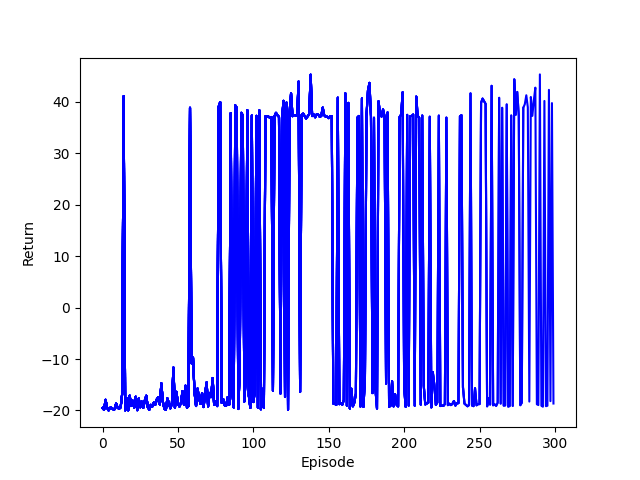
\includegraphics[width=0.6\linewidth]{dqn_training.png}
\end{figure}

\subsection{Política Aprendida pelo DQN}

\begin{figure}[!h]
    \centering
    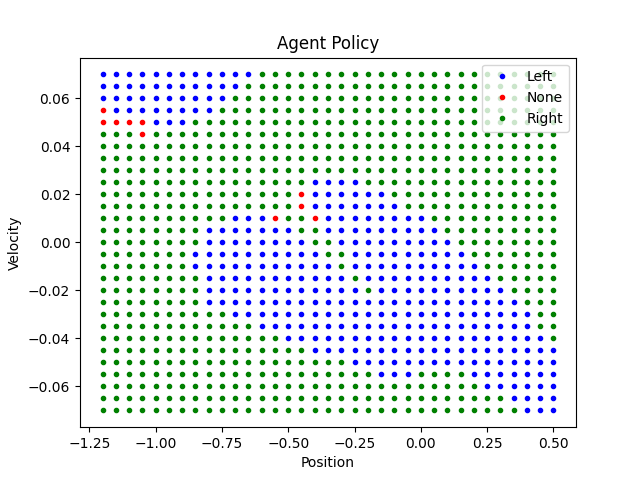
\includegraphics[width=0.6\linewidth]{agent_decision.png}
\end{figure}

\newpage

\subsection{Retorno de 30 Episódios Usando a Rede Neural Treinada}

\begin{figure}[!h]
    \centering
    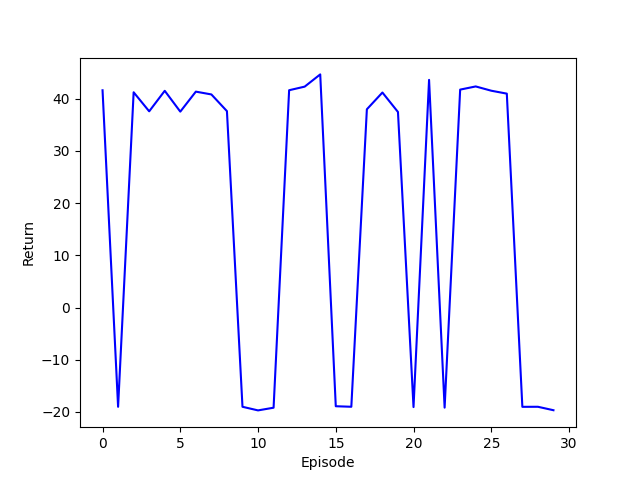
\includegraphics[width=0.6\linewidth]{dqn_evaluation.png}
\end{figure}

\section{Discussão dos Resultados}

Durante os 30 episódios de avaliação, o agente obteve desempenho satisfatório em 18 deles, correspondendo a uma taxa de sucesso de 60\%. Esses episódios foram caracterizados por pontuações positivas, indicando que o objetivo do ambiente foi alcançado com sucesso. Nos demais 40\% dos episódios, o agente falhou em atingir o objetivo dentro do tempo máximo permitido, resultando em pontuações negativas próximas de $-19$.

O retorno médio ao longo dos episódios foi de aproximadamente $18.80$, valor impactado negativamente pelas penalidades acumuladas nos episódios malsucedidos. Observa-se uma contradição entre episódios de alto desempenho e episódios com falha total, o que sugere que a política aprendida ainda apresenta instabilidade. Esse comportamento pode estar relacionado à generalização incompleta da política treinada.

No geral, embora o agente tenha demonstrado capacidade de resolver a tarefa em uma parte significativa dos episódios, um maior treinamento e refinamento das estratégias de aprendizado ainda podem ser usados para melhorar o desempenho do agente.
\end{document}